\documentclass[11pt]{article}

\usepackage{geometry}
\geometry{letterpaper, margin=1in}

\usepackage{graphicx}
\usepackage{booktabs}
\usepackage{amsmath}
\usepackage{natbib}
\usepackage{caption}
\usepackage{hyperref}
% Setup hyperref properties
\hypersetup{
  pdftitle={Cultural Matching and the Persistence of Social Ties},
  pdfauthor={Michael Lee Wood, David Hachen, Brandon Sepulvado, Omar Lizardo},
  colorlinks=true,
  linkcolor={blue},
  filecolor={maroon},
  citecolor={blue},
  urlcolor={blue}
}

\title{Do Birds of a Father Flock Together? Examining Religious Homophily Dynamics at a Catholic University}
\author{
  Michael Lee Wood \\ \textit{Brigham Young University} \and
  David Hachen \\ \textit{University of Notre Dame} \and
  Brandon Sepulvado \\ \textit{NORC at the University of Chicago} \and
  Omar Lizardo \\ \textit{UCLA}
}
\date{\today}

\begin{document}

\maketitle
\newpage
\begin{abstract}
Traditional homophily indices often conflate individual preferences with baseline structural opportunities, creating systematic biases when comparing minority and majority groups. We address this by examining religious homophily and friendship choice using longitudinal network data from the NetHealth Cohort Study ($N = 722$ students). Using a dyadic framework with an opportunity offset, we adjust for baseline group sizes and physical and social foci, such as residential proximity and socio-demographic homophily. We find that all religious groups exhibit persistent inbreeding homophily. However, our opportunity-adjusted models reveal that non-Catholic religious affiliation, considered collectively (Protestant, No Religion, and Other Religion), has a stronger positive effect on active homophily compared to the Catholic majority, supporting Minority Distinctiveness Theory at the Catholic/non-Catholic level. A bootstrap sensitivity analysis indicates that the specific ordering of effects among the three non-Catholic groups is not statistically reliable, and should not be interpreted as evidence of a fine-grained distinctiveness hierarchy.
\end{abstract}

\newpage
\section{Introduction}
\subsection{Background}
How does the numeric composition of a local social environment shape the formation of friendship ties across religious groups? While the reliable tendency for individuals to associate with similar others---homophily---is one of social science's most well-established empirical generalizations \citep{mcpherson2001}, explaining \textit{why} different groups exhibit varying degrees of homophily within a given population remains an open question \citep{mcfarland2014network-735}. Although selectively forming ties with similar others can be an individual choice, it is also influenced by structural factors such as propinquity, opportunity structure, and social foci \citep{rivera2010dynamics-e3e, feld2009}. In this regard, network analysts distinguish between ``choice homophily'' resulting from individual preferences and ``induced homophily'' resulting from structural processes such as uneven group sizes or physical proximity \citep{kossinets2009, mcpherson2001, marsden1988, hofstra2017sources-be0}. Furthermore, structural clustering can emerge via ``consolidation'' or multiform heterogeneity \citep{blau1977book}, in which preferences for similarity along one dimension (e.g., gender or dormitory) narrow the pool of available alters, thereby indirectly altering apparent homophily along other dimensions. 

A subset of structural theories of homophily focuses on how the uneven distribution of group sizes creates motivational (dis)incentives and a biased opportunity structure landscape for forming same-group and out-group ties. In this regard, there are two explanations for how relative group size intersects with homophily (and heterophily) generating processes. 

Under the \emph{Minority Distinctiveness Hypothesis} (MDH), a numeric minority status increases the cognitive salience of that group identity in the context of outgroup numerical dominance, which is theorized to produce active sorting patterns consistent with minority members banding together to preserve their subcultural boundaries \citep{mehra1998, leonard2008, marsden1988, sepulvado2015}. 

Conversely, following Blau's classic treatment, what we might refer to as the \emph{Majority Exclusiveness Hypothesis} (MEH) suggests that a dominant majority possesses the structural and social leverage to guard group boundaries, which means that they should exhibit stronger tendencies towards homophily, doubly aided by their standing as more numerous and more readily available tie-formation partners (majority members are more numerically available) and ``induced'' (there are more members of the majority to choose from) considerations. As Blau observed, ``the larger of two groups discriminates more than the smaller against associating with members of the other group,'' resulting in higher active homophily among the majority \citep[p.~81]{blau1977book}.

\subsection{Study Setting}
An ideal setting for examining the MDH and MEH predictions would be a highly specific network ecology in which a single group holds overwhelming numerical dominance. The University of Notre Dame (ND) presents such a unique social laboratory for the present research \citep{hachen2022generators-923}. 

In the \textit{NetHealth Study}'s \citep{purta2016experiences-7de} longitudinal cohort, Catholic students represent approximately $72.7\%$ of the student body, while Protestant ($9.8\%$), non-religious ($12.3\%$), and other religious students ($4.6\%$) constitute small, distinct minorities. However, this setting introduces a profound institutional focus \citep{feld1981, feld2009}: religion is not merely a demographic attribute; it defines the university's very identity and physical infrastructure. Crucially, Catholics attending a Catholic university might be more motivated to befriend other Catholics because the environment ``summons'' their religious identity, increasing its salience \citep{tavory2016}. Furthermore, ND features built-in residential and social foci---such as single-sex dormitories, mandatory dorm assignments, and Catholic-oriented campus activities---that could organically channel Catholics into homophilous friendships without requiring any active individual preference for Catholic friends; our tie-formation data cannot itself establish whether such preferences are also present, only whether observed mixing patterns exceed what these structural mechanisms would predict on their own.

To evaluate the predictions of the MDH (higher homophily rates among minorities) versus the MEH (higher homophily rates among the majority), it is important to move beyond the limitations of raw homophily rates and aggregate indices. Traditional aggregate measures, such as Krackhardt's E-I (External-Internal) index \citep{krackhardt1988informal-42d}, suffer from a well-known artifact: in a bounded network, a numeric minority is structurally forced to have higher outgroup contact, regardless of their personal preferences, a phenomenon also emphasized by \citet{blau1977}, thus producing a form of ``induced heterophily.'' Consequently, aggregate comparisons are biased \citep{everett2012categorical-592}. Here, we address that issue by transitioning to a dyadic (tie-level) framework with an opportunity offset. This approach allows us to adjust for baseline group sizes in the data, as well as other important drivers of homophily, such as physical propinquity and social foci, as well as other forms of homophily beyond the focal one in our study. 

To this end, this paper leverages 8 waves of longitudinal network data from the \textit{NetHealth Study} to examine the trajectory of religious homophily. We test whether the observed homophily of Protestants and other religious minorities is merely a byproduct of residential sorting and alternative tie-level demographic similarities, or whether it reflects a recurrent, active sorting process consistent with the identity-salience mechanism amid Catholic numerical dominance, as proposed by the MDH. Our tie-level data can establish whether mixing patterns exceed what structural and demographic explanations predict, but cannot directly observe salience or preference as psychological states.

\section{Methods and Data}

\subsection{Data Source and Sample Design}
We evaluate the dynamics of religious homophily and friendship choice using longitudinal social network and survey data from the \textit{NetHealth Study} at the University of Notre Dame, a multi-year, NIH-funded data-collection project. \textit{NetHealth} tracked a single cohort of undergraduate students from their entry as freshmen in Autumn 2015 through their graduation in Spring 2019. Initial recruitment enlisted around 700 students (yielding a total sample of $N = 722$ participants who took at least one survey), representing roughly $36\%$ of the typical incoming freshman cohort. While this is an exceptionally high coverage rate for an intensive longitudinal ego-network study, the multi-tiered recruitment strategy (which included snowball sampling) may introduce selection bias into homophily estimates if students systematically recruited highly similar alters into the study. The project tracked their social networks, behaviors, and attributes over 8 waves of data collection fielded approximately every 3--4 months. 

In each of the eight waves, respondents completed a name-generator survey with the prompt: ``We would like to know who you consider to be in your social network. In the spaces below, please list up to 20 people with whom you spend time communicating or interacting.'' Beginning with Wave 3, respondents were presented with their previously nominated alters and were allowed to add up to 5 more, for a maximum of 25 alters. These name generators, coupled with name interpreters detailing each alter's characteristics and the nature of the relationship, yielded a unique multiwave, long-term ego-network dataset that constitutes our primary data source. For the purposes of evaluating within-cohort homophily, we restrict alter nominations to those designated as fellow on-campus students.

\subsection{Variables}

\subsubsection{Ego-Level (Participant) Measures}
Ego-level attributes are drawn from the \textit{NetHealth} Basic Survey, which captured demographic and behavioral characteristics across the eight waves. Baseline traits were measured at Wave 1. The primary independent variable is baseline \textit{ego religion}. Respondents were categorized into four groups: Catholic ($72.7\%$, the dominant majority), No Religion ($12.3\%$), Protestant ($9.8\%$), and Other Religion ($4.6\%$). Missing responses account for $<1\%$. Additional demographic controls include \textit{ego gender}, coded as Woman ($51.1\%$) or Man ($47.9\%$), and \textit{ego race/ethnicity}, categorized into White ($65.0\%$), Latino/a ($12.3\%$), Asian-American ($8.7\%$), Foreign Student ($7.1\%$), African-American ($5.7\%$), and Other ($<1\%$). To control for individual-level \textit{religious salience (frequency of discussion)} independent of homophily, we use a measure of how frequently the respondent discusses religion (captured in Wave 2). Responses are recorded on a 5-point Likert scale ranging from ``Not at all'' ($4.6\%$), ``Less than 1-2 times a month'' ($11.8\%$), ``1-2 times a month'' ($31.9\%$), ``1-2 times a week'' ($27.4\%$), to ``Three times a week or more'' ($12.6\%$).

\subsubsection{Alter-Level (Tie) Measures}
Alter characteristics and relationship contexts are derived from the \textit{NetHealth} Network Survey, in which egos provided information about their nominated peers. For the \textit{alter relationship context}, denoting the relation of the alter to the university (e.g., Student, Alum, Prospect), $48.6\%$ of overall nominations were for fellow students. We subset our dyadic data to these alters ($N = 17,452$ student ties). Egos reported the perceived \textit{alter religion} of each nominated fellow student (Catholic: $67.8\%$; Protestant: $6.8\%$; No Religion: $7.2\%$; Other Religion: $2.2\%$; Missing: $15.9\%$). This is used to construct our primary outcome variable, a binary indicator of religious homophily (coded $1$ if ego and alter share the same religious affiliation, and $0$ otherwise). Egos also reported each student \textit{alter gender and race} (e.g., Woman: $52.2\%$; Man: $47.8\%$, and White: $78.0\%$). These allow us to construct binary dyadic indicators for gender homophily and racial/ethnic homophily. To adjust for structurally induced clustering, egos indicated whether each fellow student shared \textit{physical and social foci (roommates and dorms)}, noting whether the alter was a roommate ($13.6\%$ yes) and whether they resided in the same dormitory ($34.9\%$ yes).\footnote{At Notre Dame, the dormitory system constitutes a primary axis of residential and social life.} Finally, egos were asked to report how close they felt to each nominated alter on an ordered scale of \textit{friendship closeness (intimacy)}. We construct an ordered numeric indicator for friendship intensity (coded 1 for ``Distant'', 2 for ``Less Than Close'', 3 for ``Merely Close'', and 4 for ``Especially Close''). This continuous indicator is added to our multivariate models to control for baseline differences in the homophily of strong versus weak ties.

\subsection{Opportunity Offset Formulation}

To model the likelihood that a tie is homophilous on religion while adjusting for baseline group proportions, we employ a dyadic logistic regression with an opportunity offset \citep{scott_wild91}. In highly skewed settings like Notre Dame, where Catholics make up nearly three-quarters of the student body, a traditional regression approach struggles to separate active friendship preferences from simple numeric availability. A Catholic student is highly likely to befriend another Catholic simply because the vast majority of their available peers are Catholic \citep{blau1977}, not necessarily because they are actively seeking out a same-religion friend. The opportunity offset corrects for this by subtracting the baseline probability of meeting someone of the same religion under conditions of random mixing.

Formally, we specify the model as:

\begin{equation}
\operatorname{logit}(P(\text{Same Religion} = 1)) = \beta_0 + \beta_1 \text{EgoReligion} + \mathbf{X}\mathbf{\beta} + \text{opportunity\_offset}
\end{equation}

In this equation, the $\text{opportunity\_offset}$ is defined as $\log\left(\frac{p_w}{1 - p_w}\right)$, where $p_w$ represents the overall proportion of the respondent's religious group in the available pool of peers for that specific wave. By forcing this term into the model with a fixed coefficient of $1.0$, we adjust the baseline odds of tie formation. Consequently, the remaining coefficients represent the \textit{excess} tendency to form a homophilous tie above and beyond what the structural opportunity pool dictates.

The model also includes $\mathbf{X}$, a vector of dyadic controls representing alternative mechanisms that might induce homophily without active religious sorting. These include demographic similarities (same gender and same race) as well as physical and social foci (being roommates or living in the same dorm). This specification provides a direct test of the MDH and MEH predictions. A positive $\beta_1$ coefficient for a minority group indicates that the group exhibits significantly stronger religious homophily than the Catholic majority, even after accounting for their smaller population size and alternative sorting mechanisms. Such a result would directly support the MDH, demonstrating that numeric minorities actively forge tighter in-group bonds in response to a dominant-majority environment.

\subsection{Methodological Advantages of the Dyadic Approach}

\subsubsection{Benefits of the Opportunity Offset}

The Krackhardt and Stern (1988) External-Internal (E-I) index is defined as $EI = (E - I) / (E + I)$. Under random mixing, the expected E-I index for group $G$ is a direct linear function of group size $p$:

\begin{equation}
EI_{\text{expected}} = (1 - p) - p = 1 - 2p
\end{equation}

Because the baseline shifts with $p$, raw E-I indices cannot be compared across groups of different sizes to infer preferences. Individual-level aggregations of normalized E-I indices also introduce a severe boundary bias: any minority ego with zero same-religion ties is assigned an $EI_{\text{norm}}$ of exactly $+1.0$. Averaging these individual scores heavily pulls the minority group's average toward $+1.0$, falsely indicating heterophily. Our dyadic logistic regression with an opportunity offset ($\log(p/(1-p))$) mitigates these biases. Entering this offset with its coefficient constrained to exactly $1.0$ subtracts the baseline opportunity structure. Consequently, the model intercept and group coefficients represent the \textit{excess log-odds of homophilous tie formation beyond what is expected under random mixing}, providing a control-integrated point estimate that is not subject to the E-I index's boundary and aggregation biases. This addresses bias in the point estimate itself; it does not guarantee that coefficients are equally \textit{precise} across groups of very different sizes. As our Results show, groups with few unique egos (e.g., Other Religion) yield coefficients with substantially wider uncertainty, which limits how confidently their magnitude can be compared to other groups' even though the point estimates themselves are not systematically biased by group size.

\subsubsection{Why Dyadic Clustered Regression is Preferable to Mixed-Effects Multilevel Models}

In social network analysis, egocentric network datasets are inherently hierarchical: nominated friendship ties (Level-1) are nested within individual egos (Level-2 clusters). To correct for this nesting, methodologists frequently recommend mixed-effects logistic regressions:

\begin{equation}
\log\left(\frac{P(Y_{ij} = 1 \mid \gamma_i)}{1 - P(Y_{ij} = 1 \mid \gamma_i)}\right) = \beta_0^C + \beta_1^C \text{EgoReligion}_i + \mathbf{\beta}_2^C \mathbf{X}_{ij} + \gamma_i + \text{offset}_{wi}
\end{equation}

Where $\gamma_i \sim N(0, \sigma^2)$ is a random intercept for ego $i$, suggesting that multilevel models can be a useful way to model this type of data \citep{snijders2003multilevel-9af}. But it can be shown that, for the purposes of answering our questions, the mixed-effects multilevel model is statistically and conceptually less appropriate than a population-average dyadic logistic regression with robust clustered standard errors. First, in a mixed-effects logistic model, the estimated fixed effects ($\beta^C$) are conditional: they represent the change in log-odds for a \textit{specific individual} if that individual's religion were to change. But if religion is a relatively stable baseline trait, as it is in our data, then this is a somewhat less-than-realistic modeling assumption. In contrast, our model with robust clustered standard errors represents a marginal (population-average) model:

\begin{equation}
\log\left(\frac{P(Y_{ij} = 1)}{1 - P(Y_{ij} = 1)}\right) = \beta_0^M + \beta_1^M \text{EgoReligion}_i + \mathbf{\beta}_2^M \mathbf{X}_{ij} + \text{offset}_{wi}
\end{equation}

Substantively, because our core hypothesis concerns group-level differences across the population, the marginal population-average model is the more appropriate approach. 

Secondly, the conditional parameters estimated by mixed-effects models are always larger in absolute value than the marginal parameters, indicating that the unobserved ego-level heterogeneity is large and that the random intercepts $\gamma_i$ act as a ``sponge,'' absorbing the unobserved cluster-level variance. This collinearity causes the fixed effects in the MLM to shrink toward zero, stripping the model of its statistical power. 

Finally, because Protestant and Other Religion students constitute relatively small percentages of the student body, the probability that a minority ego has \textit{exactly zero} same-religion friends is high. When an ego has zero same-religion friends, their Level-1 outcome $Y_{ij}$ has zero variance. In a mixed-effects logistic regression, the maximum likelihood estimate of the random intercept for an ego with zero successes is negative infinity ($\hat{\gamma}_i \to -\infty$). When the numerical solver attempts to estimate the random effects for these zero-variance clusters, the algorithm fails to find stable starting values and diverges. Our dyadic logistic regression with robust clustered standard errors avoids these numerical and conceptual pitfalls: it is numerically stable, conceptually accurate, and produces statistically defensible standard errors.

\section{Results}

\subsection{Baseline Opportunity Structure Stability}

Before analyzing active homophily, it is crucial to establish the stability of the baseline opportunity structure. If the numeric composition of the student body fluctuated wildly over the four years, any changes in tie formation could simply be an artifact of changing demographics rather than evolving social preferences. The wave-specific proportions of available student peers across Waves 3 to 8 are plotted in Figure~\ref{fig:opportunity-stability}. The extreme flatness of these lines visually confirms that the structural opportunity pool is highly stable, ensuring that the changes in homophily observed in subsequent models reflect genuine behavioral sorting rather than demographic drift.


\subsection{Longitudinal Trajectories of Religious Homophily (Yule's Q)}

To address the group-size artifact, we first evaluate the longitudinal trajectory of religious mixing using group-level, baseline-adjusted Yule's $Q$ across all eight waves of the college cohort (see Figure~\ref{fig:yules-q}). Unlike alternative aggregate metrics---such as raw in-group tie percentages, Coleman's homophily index, or Krackhardt and Stern's E-I (External-Internal) index---Yule's $Q$ is independent of relative group sizes \citep[159]{borgatti2024analyzing}. Because traditional measures like the E-I index are strictly bounded by the available opportunity pool, they inherently force numeric minorities to exhibit higher rates of heterophily simply due to their small baseline population, distorting cross-group comparisons \citep[for a review mapping segregation measures to theoretical properties, see][]{bojanowski2014}. 

In contrast, Yule's $Q$ is a direct transformation of the odds ratio, rendering it margin-free: unlike the E-I index, its expected value under random mixing is $0$ regardless of group size. This makes Yule's $Q$ well suited to testing, \textit{within each group}, whether observed mixing departs from what that group's own random-mixing baseline would predict.\footnote{In supplementary analyses, we confirmed that these results are robust to alternative specifications, including point-biserial correlation coefficients \citep{everett2012categorical-592}, which also show a consistent positive mean tendency for religious homophily after accounting for group-size imbalances.} Margin-invariance of the expected value does not, however, imply that raw $Q$ magnitudes are comparable \textit{across} groups of very different sizes. A degree-preserving permutation analysis (resampling alters within each wave's observed opportunity pool while holding each ego's degree fixed) shows that, for groups as small as Other Religion, the null distribution of $Q$ is itself both wide and biased away from zero, so a given raw $Q$ is far less surprising for a small group than the identical value would be for a large one. We therefore use Yule's $Q$ to establish that each group, individually, sorts more than its own chance baseline predicts, rather than to rank the relative strength of homophily across groups of unequal size.

Yule's $Q$ is defined as:

\begin{equation}
Q = \frac{ad - bc}{ad + bc}
\end{equation}

Where $a$ is the number of ingroup ties (e.g., Catholics befriending Catholics), $b$ is the number of outgroup ties from group $G$ (Catholics befriending non-Catholics), $c$ is the number of ties from the outgroup to group $G$ (non-Catholics befriending Catholics), and $d$ is the number of ties strictly between outgroup members (non-Catholics befriending non-Catholics). 

The resulting index ranges from $-1$ to $+1$. A value of $0$ indicates perfect random mixing, in which ties form without regard to religion. A positive value ($Q > 0$) indicates ``inbreeding homophily'' \citep{marsden1988}: an excess of same-group ties relative to what random mixing would predict, consistent with active sorting toward same-group friends. At the extreme, a $Q$ of $+1$ implies absolute homophily, where group members only ever befriend their own kind. Conversely, a negative value ($Q < 0$) indicates heterophily: an excess of cross-group ties relative to chance, consistent with active avoidance of same-group ties, with $-1$ indicating that every friendship crosses religious lines.


Our descriptive findings provide strong evidence of \textit{universal inbreeding homophily} ($Q > 0$) for every religious group in every single wave. Over the four years of college, students consistently choose friends who share their religious affiliation at rates that exceed those expected under random mixing. Rather than relying on the raw magnitude of $Q$ alone, we anchor this claim to a degree-preserving permutation test: for each ego, we hold degree and own religion fixed and redraw nominated alters' religion from that wave's observed opportunity pool, generating a null distribution of $Q$ against which the observed value is standardized. As Table~\ref{tab:yules-q-null} shows, every group's observed $Q$ exceeds its own permutation null in every wave ($z$-scores range from 1.3 to 7.5, $p < 0.05$ in all but one group-wave combination). This test speaks only to whether each group, individually, departs from its own chance baseline; it is not a basis for ranking groups against one another, since a group's null variance itself scales with its size. Any claims about the relative strength of homophily across religious groups are addressed separately, and with appropriate caveats, in the dyadic regression results below.

\subsection{Opportunity-Adjusted Cross-Sectional Regressions (Wave 3)}

We fit three nested dyadic logistic regression models to Wave 3 student nominations (sophomore-year baseline), adjusting for various tie-level covariates, including physical propinquity (e.g., residing in the same dorm) and gender and race homophily. As Table~\ref{tab:wave3-reg} shows, the nested models reveal that \textit{non-Catholic students collectively exhibit significantly stronger opportunity-adjusted homophily than the Catholic majority, whose own baseline coefficient is not reliably distinguishable from zero}. When controlling for roommates, dormitory co-residence, gender homophily, and race homophily matching in Model 2, the Protestant ($\beta = 0.599, p < 0.01$), Other Religion ($\beta = 1.898, p < 0.001$), and No Religion ($\beta = 0.577, p < 0.05$) coefficients are all positive and remain stable. Model 3 shows that this pattern persists after adjusting for individual-level religious salience (frequency of discussing religion), indicating that the elevated non-Catholic homophily is not simply a byproduct of minority students being more religious.

We caution against over-interpreting the relative magnitude of these three coefficients as evidence of a fine-grained ranking among non-Catholic subgroups. The Other Religion group comprises only 16 egos and 55 dyads at Wave 3, and a bootstrap resampling analysis at the ego level (resampling egos with replacement within each religious group, holding the wave-specific opportunity pool fixed) shows that its excess in-group tie rate is not statistically distinguishable from that of Protestant or No Religion students---the pairwise 95\% confidence intervals for all three minority-minority contrasts include zero. The large point estimate for Other Religion on the logit scale is consistent with its small denominator rather than demonstrable evidence of a comparatively stronger preference for in-group ties. We therefore treat these results as evidence that non-Catholic religious affiliation, considered collectively, is associated with elevated opportunity-adjusted homophily relative to the Catholic majority, without treating the specific ordering of coefficients across non-Catholic subgroups as a reliable finding.

While such a reduction in nested nonlinear models is often casually interpreted as a mediation effect---suggesting that secular clustering is ``explained away'' by structural foci like dorms or demographics---this is problematic. In logistic regression, adding covariates rescales the error-term variance, rendering coefficient comparisons across nested models invalid (often called the rescaling or unobserved heterogeneity problem). To determine if physical and demographic foci genuinely mediate the No Religion effect, we conducted a formal causal mediation analysis using the \texttt{mediation} package in R \citep{imai2010}. The formal analysis reveals that the Average Causal Mediation Effects (ACME) for these covariates are all statistically indistinguishable from zero (e.g., $p = 0.32$ for same-dorm co-residence and $p = 0.16$ for race homophily matching). Thus, rather than secular homophily being structurally mediated, the No Religion coefficient's stability across Models 1--3 in Table~\ref{tab:wave3-reg} ($\beta = 0.698, 0.660,$ and $0.577$, respectively, all $p < 0.05$) reflects a genuine, direct association that is not explained away by physical or demographic sorting.

\subsection{Pooled Longitudinal Regressions with Robust Clustered Standard Errors}

To trace how these associational boundaries evolve longitudinally throughout the college career, we fit a pooled interaction model across Waves 3–8 (Table \ref{tab:pooled-interaction-reg}). Because individual students are observed repeatedly, we estimate robust standard errors clustered at the respondent level. The results, summarized in Table \ref{tab:pooled-interaction-reg}, show that the No Religion group also exhibits a statistically significant positive effect on active homophily ($\beta = 0.576, p < 0.01$) when pooled across all waves, consistent with the significant, stable No Religion coefficient already observed across all three Wave 3 cross-sectional models. Furthermore, we find a counter-intuitive negative effect of same-dorm co-residence on the probability of forming a same-religion tie ($\beta = -0.249, p < 0.05$). We also observe significant racial dynamics: ego-level race effects show that students identifying as African-American form religious homophilous ties at higher rates than White students,\footnote{This finding is likely partially driven by the religious composition of the student body: African-American students in our sample are significantly more likely to be Protestant ($29.3\%$) compared to White students ($7.9\%$), and since Protestant students at this institution exhibit high levels of active homophily, the race coefficient partially captures this religious effect.} while race homophily (the dyadic tendency to bond with same-race peers) is also a strong, significant predictor of network cohesion ($\beta = 0.433, p < 0.001$), indicating that religious and racial boundaries operate as complementary, rather than competing, axes of social sorting. The results also show that \textit{non-Catholic groups collectively maintain an elevated, opportunity-adjusted homophily relative to the Catholic majority that does not change appreciably over time}, as evidenced by broadly parallel trends across waves. As with the Wave 3 results, we caution against reading the specific magnitudes across Protestant, No Religion, and Other Religion as a stable ranking. A pooled bootstrap analysis across Waves 3--8 (resampling the 473 unique egos who contribute ties, respecting within-ego clustering across waves) confirms that Protestant and No Religion students each show a modest but statistically robust excess in-group tie rate relative to Catholics (approximately 6--10 percentage points above the chance baseline), but Other Religion---limited to only 22 unique individuals across the entire six-wave panel---remains statistically indistinguishable from every other group, including the Catholic majority. This indistinguishability persists after pooling six waves of data because the binding constraint is the number of distinct people in the group, not the number of observed ties: additional waves largely add repeated observations from the same small set of individuals rather than new independent information.

To evaluate these temporal interaction effects within a non-linear logit framework \citep{mize2019best-752}, we calculate and plot the marginal effects for each religious group relative to the Catholic baseline. Because raw probabilities are inherently confounded by unequal group sizes (the group-size artifact), we compute these marginal effects on the probability scale while holding the opportunity offset constant at $0$. This analytically simulates an ``equal opportunity'' scenario in which each group has an identical $50\%$ representation in the population, thereby isolating the excess probability of an active homophilous tie. To further illustrate this stability, Figure \ref{fig:active-coefs} plots the wave-specific active homophily coefficients estimated from identical cross-sectional, opportunity-adjusted logistic regressions (similar to Model 1 in Table \ref{tab:wave3-reg}). The resulting plot highlights a durable separation between the Catholic majority and non-Catholic groups collectively, maintained consistently over the course of college. The relative ordering among the three non-Catholic groups visible in the figure should not be read as a reliable ranking, given the small and uneven sample sizes underlying the Protestant, No Religion, and especially Other Religion estimates.

\section{Discussion and Concluding Remarks}

Our results provide support for the MDH relative to the MEH predictions when religious groups are considered at the Catholic/non-Catholic level, though not for a finer-grained ranking among non-Catholic subgroups. The baseline homophily of the Catholic majority is largely structural---a byproduct of their sheer numeric availability within the university environment, consistent with the more streamlined version of Blau's \citeyearpar{blau1977} macro-structural theory: its opportunity-adjusted coefficient is not reliably distinguishable from zero. Because Catholics constitute nearly three-quarters of the student body, random mixing naturally yields highly homophilous networks. In contrast, non-Catholic students collectively exhibit opportunity-adjusted homophily above chance. Surrounded by a dominant majority, their minority identity may be made more salient, which could prompt more active maintenance of social boundaries around subcultural beliefs and practices. However, as detailed above, our data cannot reliably differentiate whether Protestants, students with no religion, or students of other religions exhibit a stronger version of this tendency than one another: the Other Religion group's large point estimate reflects a denominator of only 16 egos at Wave 3 (22 pooled across all waves), and a bootstrap sensitivity analysis finds no statistically reliable differences among the three non-Catholic groups. We therefore interpret the evidence as supporting a Catholic/non-Catholic distinction in active homophily rather than a specific ordering among minority religious groups.

Crucially, our revised methodological framework changes the theoretical conclusions regarding secular students (the "No Religion" group) relative to prior work relying on raw metrics or naively-scaled nested logistic regressions, which casually interpreted a drop in the secular homophily coefficient upon the introduction of spatial controls as evidence that secular clustering was merely a byproduct of physical dorm sorting. Our formal causal mediation analysis rules this out directly: the No Religion coefficient remains positive and statistically significant across every Wave 3 specification ($\beta = 0.698$ to $0.577$, $p < 0.05$ in all three models) and in the pooled longitudinal model ($\beta = 0.576, p < 0.01$), and the ACME estimates for physical and demographic foci are statistically indistinguishable from zero. Together, these results indicate that secular students' tendency toward same-group friendship is a stable, genuine association rather than an artifact of dormitory or demographic sorting--consistent with the broader finding that non-Catholic groups collectively exhibit opportunity-adjusted homophily beyond chance. Additionally, the negative effect of the same-dorm covariate suggests that within residential dorm units, the ``integrating forces'' of university life may pull students across religious lines more generally, even though they do not account for the No Religion group's persistent in-group tendency specifically.

Furthermore, our longitudinal interaction models, evaluated via marginal effects on the equal-opportunity probability scale, suggest that this elevated non-Catholic homophily is durable throughout the college career: the elevated rate of active homophily among non-Catholic students, considered collectively, does not appear to diminish or assimilate over the four years of college. These groups maintain broadly parallel and stable trajectories of in-group affinity relative to the Catholic baseline, despite the potential integrating forces of shared university spaces and randomized residential dorm assignments. As noted above, however, the data cannot support claims about which specific non-Catholic group maintains the most durable boundary.

Finally, we note several limitations of the current study. First, there is a substantial selection effect inherent to our sample: non-Catholic students have actively chosen to attend a Catholic university. As a result, they may be less culturally distinct from the Catholic majority than they would be in a secular setting, which may attenuate the boundaries we observe and shift the baseline mechanics of out-group exclusion. Second, because alter attributes are ego-reported, measurement error may be present. In a setting where Catholicism is dominant, respondents who do not know a friend's religion might assume that they are Catholic, potentially artificially inflating Catholic homophily or cross-group ties toward Catholics. Third, we observe a single institutional context with one specific distribution of religious groups. As previous research has shown \citep{goodreau2009}, the strength of homophily can vary contextually, often exhibiting curvilinear relationships with group proportions rather than strictly linear responses to minority or majority status. Future work extending these findings across multiple institutional contexts could yield greater theoretical specificity regarding the separable effects of group size and group proportion.

\newpage
\bibliographystyle{apalike}
\bibliography{references}

\newpage
\begin{table}[htbp]
\caption{\label{tab:wave3-reg}Nested Dyadic Logistic Regressions Predicting Same-Religion Ties (Wave 3).}
\centering
\scriptsize
\resizebox{\textwidth}{!}{%
\begin{tabular}[t]{lllll}
\toprule
  & Model 1 & Model 2 & Model 3 & Model 4\\
\midrule
Intercept & 0.148* (0.069) & -0.057 (0.364) & 0.031 (0.454) & -0.220 (0.625)\\
 \\ 
Ego: No Religion & 0.698*** (0.210) & 0.164 (0.267) & 0.147 (0.269) & 0.128 (0.270)\\
Ego: Other Religion & 2.044*** (0.356) & 2.076*** (0.361) & 2.062*** (0.361) & 2.087*** (0.362)\\
Ego: Protestant & 0.631** (0.193) & 0.600** (0.199) & 0.589** (0.200) & 0.625** (0.201)\\

Tie: Gender Homophily & --- & 0.073 (0.197) & 0.081 (0.200) & 0.060 (0.201)\\
Tie: Race Homophily & --- & 0.184 (0.137) & 0.170 (0.140) & 0.176 (0.140)\\
Tie: Roommates & --- & -0.245 (0.172) & -0.268 (0.173) & -0.255 (0.174)\\
Tie: Same Dorm & --- & -0.275 (0.184) & -0.307 (0.186) & -0.292 (0.187)\\
Tie: Subjective Closeness & --- & 0.080 (0.098) & 0.076 (0.099) & 0.092 (0.100)\\
Ego: Religious Salience & --- & --- & -0.011 (0.068) & -0.019 (0.069)\\
Ego: Activity (log out-deg.) & --- & --- & --- & 0.195 (0.140)\\
Alter: Popularity (log in-deg.) & --- & --- & --- & -0.297 (0.178)\\
\midrule
\multicolumn{5}{l}{\textit{Group sample sizes (unique egos / dyadic ties)}}\\
Catholic & 264 / 1,555 & 252 / 1,498 & 247 / 1,471 & 247 / 1,471\\
No Religion & 35 / 192 & 25 / 166 & 25 / 166 & 25 / 166\\
Other Religion & 16 / 55 & 15 / 54 & 15 / 54 & 15 / 54\\
Protestant & 39 / 222 & 36 / 210 & 36 / 210 & 36 / 210\\
\bottomrule
\multicolumn{5}{l}{\rule{0pt}{1em}\textit{Note:} $^{*} p < 0.05$; $^{**} p < 0.01$; $^{***} p < 0.001$}\\
\multicolumn{5}{p{0.98\textwidth}}{\footnotesize Sample sizes decline slightly from Model 1 to Models 2--4 due to listwise deletion on structural, salience, and degree covariates. The Other Religion group's small N (15--16 egos) implies substantially lower precision for its coefficient than for the other groups; see Results for a bootstrap sensitivity analysis. Model 4 adds each ego's log out-degree (number of alters nominated that wave, capturing overall gregariousness/activity) and each alter's log in-degree (number of times nominated that wave, capturing popularity), computed from the full Wave 3 nomination roster (Reviewer 1). Neither term meaningfully attenuates the Other Religion or Protestant coefficients, and No Religion is already statistically indistinguishable from the Catholic baseline once structural controls are added at Model 2, independent of degree.}\\
\end{tabular}
}
\end{table}


\newpage


\newpage
\begin{table}[htbp]
\caption{\label{tab:pooled-interaction-reg}Primary Analysis: Pooled Longitudinal and Interaction Models (Waves 3-8, Clustered SEs).}
\centering
\scriptsize
\resizebox{\textwidth}{!}{%
\begin{tabular}[t]{lllll}
\toprule
  & Model 1 & Model 2 & Model 3 (+Degree) & Interaction (+Degree)\\
\midrule
Intercept & 0.267*** (0.065) & 0.248 (0.315) & -0.120 (0.421) & -0.104 (0.407) \\
 \\
Ego: No Religion & 0.549** (0.197) & 0.556** (0.196) & 0.550** (0.195) & 0.398 (0.233) \\
Ego: Other Religion & 1.718** (0.536) & 1.727*** (0.522) & 1.718** (0.524) & 1.735** (0.561) \\
Ego: Protestant & 0.497** (0.182) & 0.496** (0.184) & 0.496** (0.185) & 0.623** (0.229) \\
Tie: Gender Homophily & --- & 0.141 (0.138) & 0.134 (0.137) & 0.134 (0.137) \\
Tie: Race Homophily & --- & 0.235* (0.119) & 0.227 (0.118) & 0.227 (0.117) \\
Tie: Roommates & --- & -0.131 (0.108) & -0.097 (0.109) & -0.098 (0.108) \\
Tie: Same Dorm & --- & -0.249* (0.127) & -0.245 (0.127) & -0.247 (0.127) \\
Tie: Subjective Closeness & --- & -0.057 (0.076) & -0.039 (0.076) & -0.030 (0.075) \\
Ego: Religious Salience & --- & 0.032 (0.060) & 0.034 (0.060) & --- \\
Ego: Activity (log out-deg.) & --- & --- & 0.187* (0.094) & 0.197* (0.092) \\
Alter: Popularity (log in-deg.) & --- & --- & -0.191 (0.126) & -0.180 (0.127) \\
Tie: Wave Number & --- & --- & --- & 0.016 (0.027) \\
Ego: No Religion x Wave & --- & --- & --- & 0.069 (0.079) \\
Ego: Other Religion x Wave & --- & --- & --- & -0.004 (0.109) \\
Ego: Protestant x Wave & --- & --- & --- & -0.057 (0.073) \\
\midrule
\multicolumn{5}{l}{\textit{Group sample sizes (unique egos / dyadic ties), Waves 3--8 pooled, fully-adjusted sample}}\\
Catholic & \multicolumn{4}{l}{326 / 7,393} \\
No Religion & \multicolumn{4}{l}{37 / 670} \\
Other Religion & \multicolumn{4}{l}{19 / 348} \\
Protestant & \multicolumn{4}{l}{46 / 1,111} \\
\bottomrule
\multicolumn{5}{l}{\rule{0pt}{1em}\textit{Note:} $^{*} p < 0.05$; $^{**} p < 0.01$; $^{***} p < 0.001$}\\
\multicolumn{5}{p{1.0\textwidth}}{\footnotesize Egos are counted once even if they contribute ties across multiple waves; standard errors clustered by egoid throughout. On-campus family ties (e.g., siblings both enrolled and nominating each other) are excluded from the analytic sample throughout, so all reported ties are nominations coded as student (non-family) relationships. Model 3 and the Interaction model add each ego's log out-degree (nominations made that wave) and each alter's log in-degree (nominations received that wave), computed from the full wave-specific nomination roster, to test whether opportunity-adjusted homophily reflects a degree/activity confound rather than affiliation itself (Reviewer 1). Neither degree term meaningfully attenuates the three group coefficients, though ego activity is itself marginally associated with same-religion tie formation ($p \approx 0.03$--$0.05$). The Other Religion group's small N (19 egos across the entire six-wave panel) implies substantially lower precision for its coefficient than for the other groups; see Results for a bootstrap sensitivity analysis.}\\
\end{tabular}
}
\end{table}


\newpage
\begin{figure}[htbp]
    \centering
    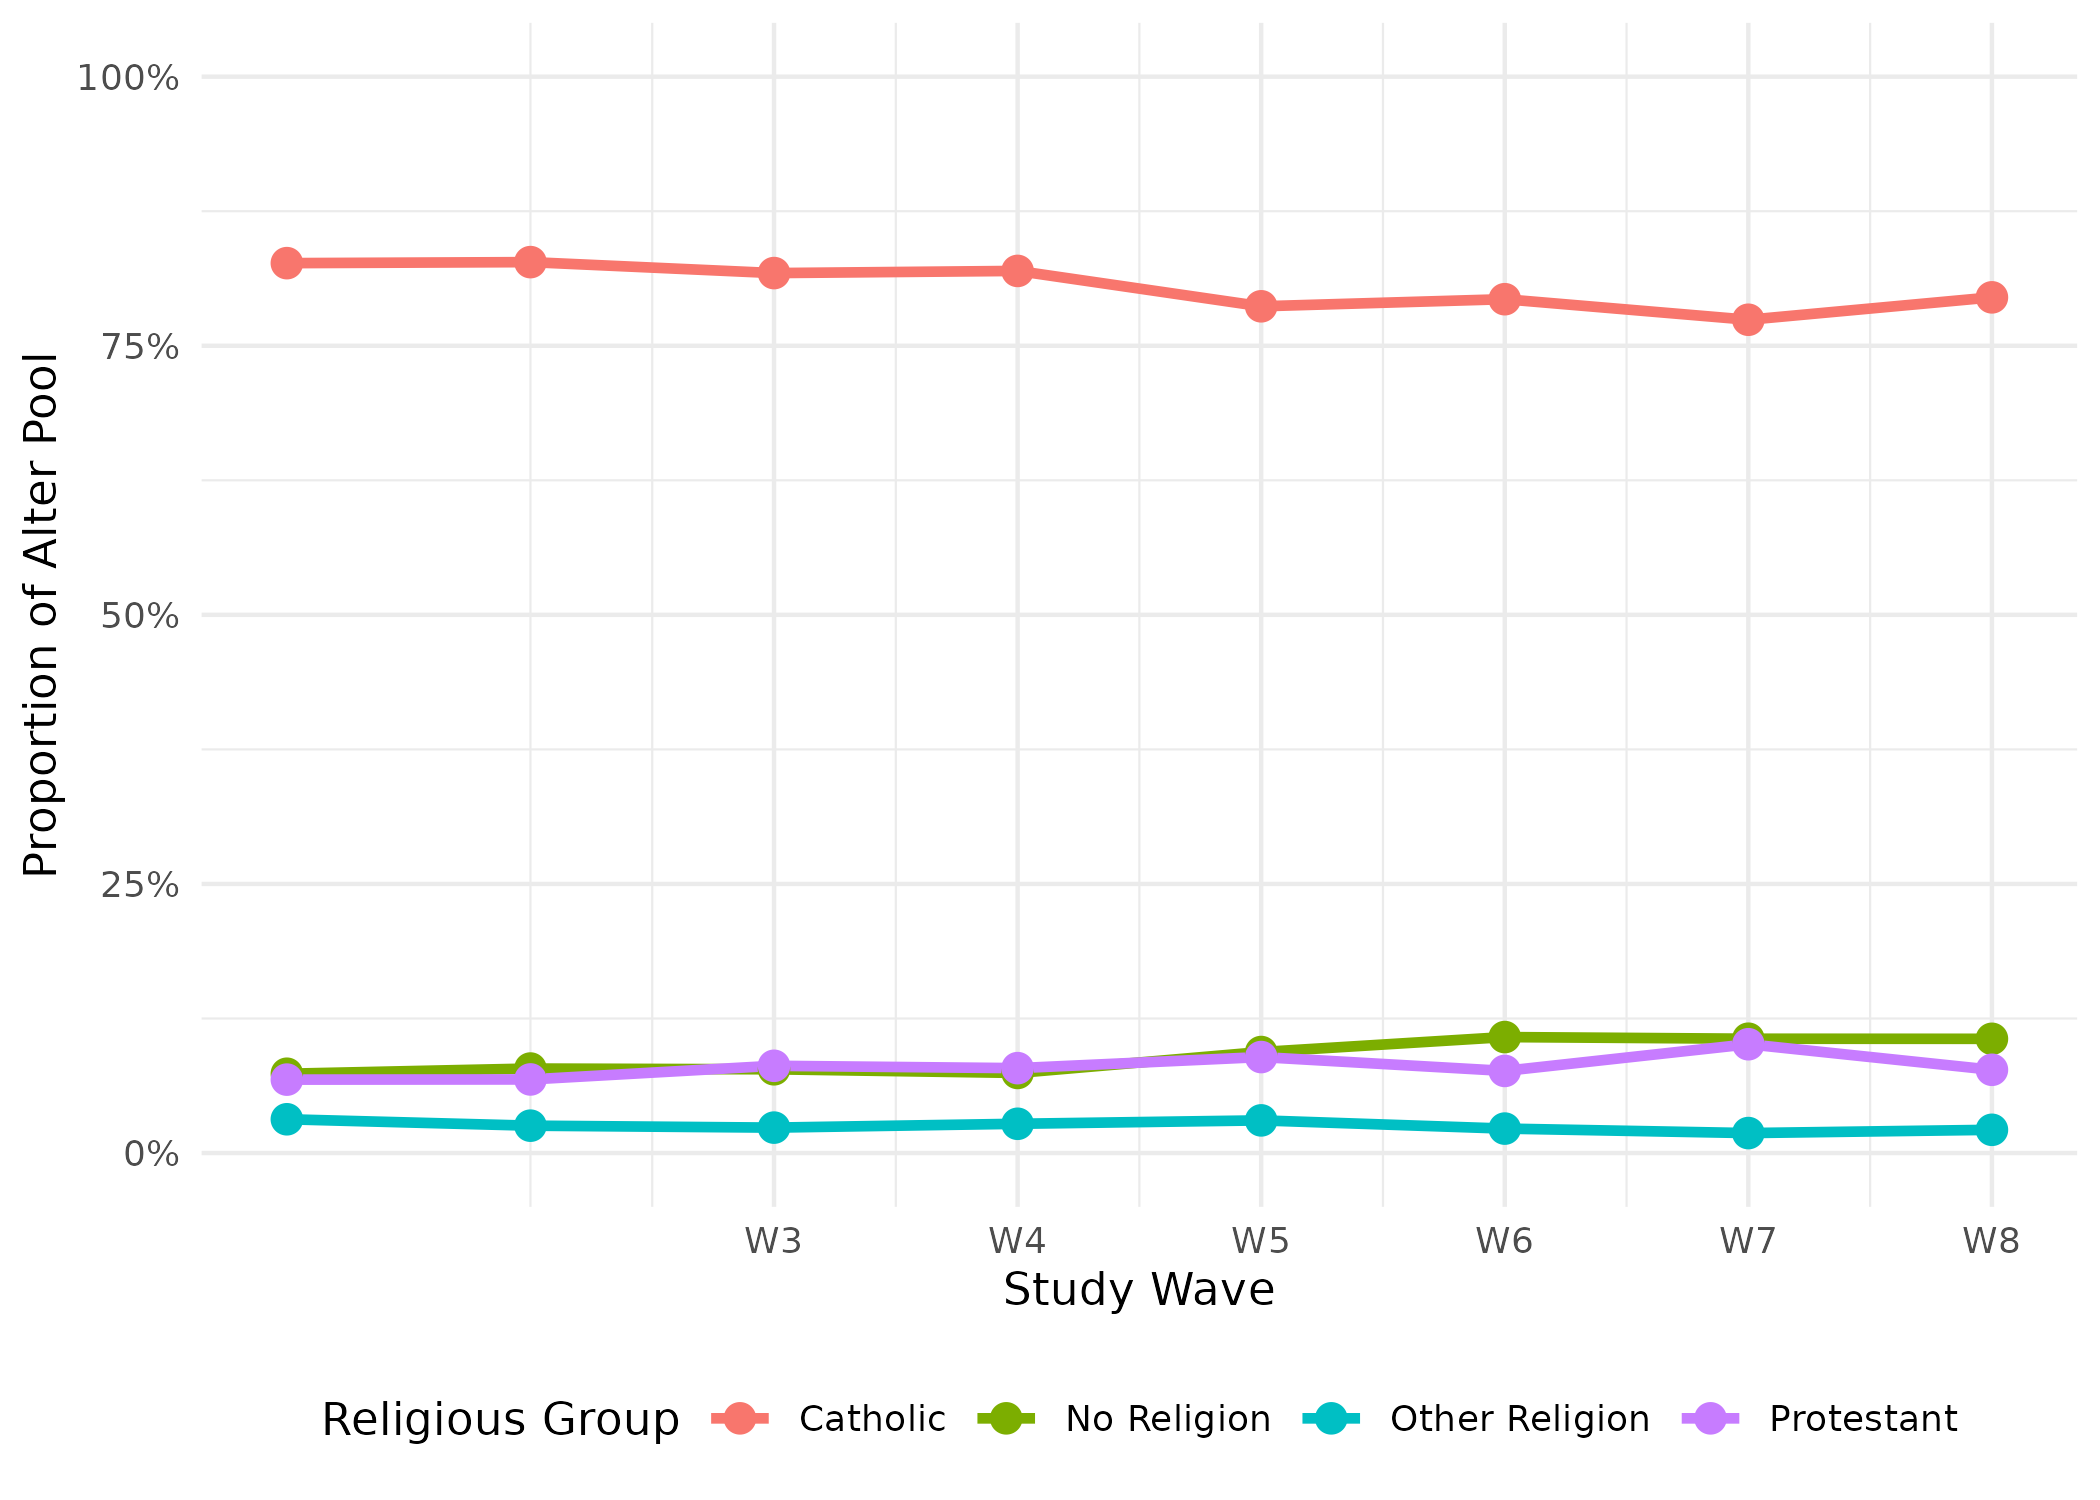
\includegraphics[width=1.0\textwidth]{Plots/fig-opportunity-stability.png}
    \caption{Religious Opportunity Structure Stability (Proportions of Available Peers, Waves 3-8).}
    \label{fig:opportunity-stability}
\end{figure}

\newpage
\begin{figure}[htbp]
    \centering
    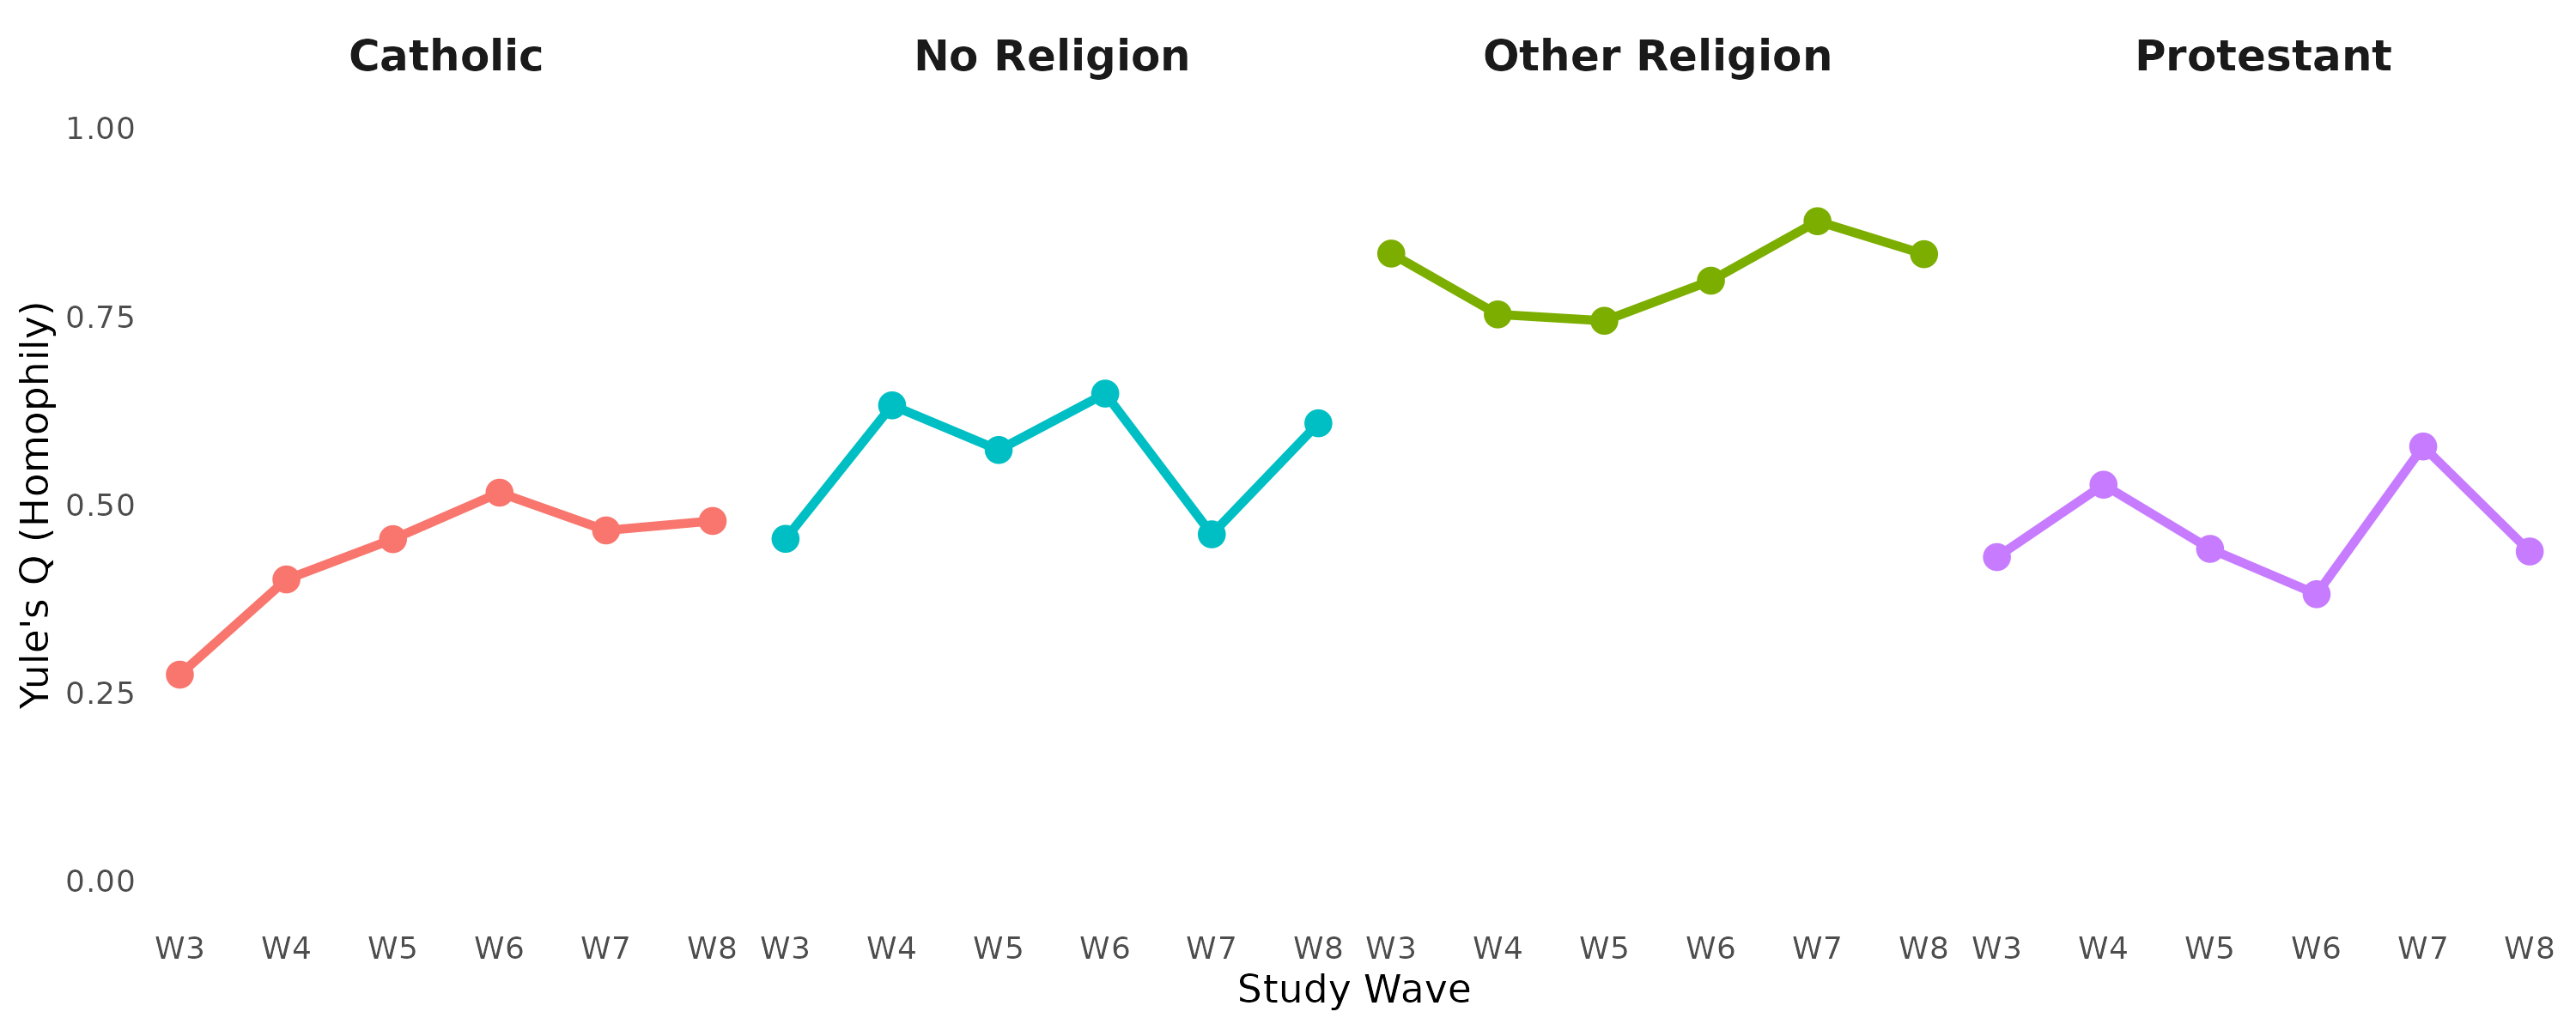
\includegraphics[width=1.0\textwidth]{Plots/fig-yules-q.png}
    \caption{Longitudinal Trajectories of Religious Homophily (Yule's Q) across Waves 3 to 8.}
    \label{fig:yules-q}
\end{figure}

\newpage
\begin{table}[htbp]
\caption{Degree-Preserving Permutation Test of Yule's $Q$ (Waves 1--8).}
\label{tab:yules-q-null}
\centering
\small
\begin{tabular}{llccccc}
\toprule
Wave & Group & Observed $Q$ & Null Mean & Null SD & $z$ & $p$ \\
\midrule
W1 & Catholic & 0.422 & -0.001 & 0.122 & 3.47 & $<$0.001 \\
 & No Religion & 0.833 & -0.026 & 0.250 & 3.44 & $<$0.001 \\
 & Other Religion & 0.726 & -0.384 & 0.688 & 1.61 & 0.016 \\
 & Protestant & 0.352 & -0.066 & 0.313 & 1.34 & 0.059 \\
\addlinespace
W2 & Catholic & 0.310 & -0.002 & 0.052 & 6.00 & $<$0.001 \\
 & No Religion & 0.530 & -0.006 & 0.100 & 5.38 & $<$0.001 \\
 & Other Religion & 0.794 & -0.089 & 0.369 & 2.40 & $<$0.001 \\
 & Protestant & 0.414 & -0.014 & 0.105 & 4.07 & $<$0.001 \\
\addlinespace
W3 & Catholic & 0.274 & -0.000 & 0.067 & 4.08 & $<$0.001 \\
 & No Religion & 0.454 & -0.018 & 0.151 & 3.12 & $<$0.001 \\
 & Other Religion & 0.833 & -0.193 & 0.528 & 1.94 & $<$0.001 \\
 & Protestant & 0.430 & -0.008 & 0.134 & 3.28 & $<$0.001 \\
\addlinespace
W4 & Catholic & 0.400 & -0.002 & 0.066 & 6.08 & $<$0.001 \\
 & No Religion & 0.632 & -0.017 & 0.157 & 4.14 & $<$0.001 \\
 & Other Religion & 0.752 & -0.105 & 0.397 & 2.16 & $<$0.001 \\
 & Protestant & 0.526 & -0.008 & 0.130 & 4.12 & $<$0.001 \\
\addlinespace
W5 & Catholic & 0.454 & -0.003 & 0.061 & 7.47 & $<$0.001 \\
 & No Religion & 0.572 & -0.018 & 0.145 & 4.09 & $<$0.001 \\
 & Other Religion & 0.744 & -0.092 & 0.354 & 2.36 & $<$0.001 \\
 & Protestant & 0.441 & -0.008 & 0.118 & 3.80 & $<$0.001 \\
\addlinespace
W6 & Catholic & 0.516 & 0.002 & 0.072 & 7.14 & $<$0.001 \\
 & No Religion & 0.647 & -0.015 & 0.148 & 4.47 & $<$0.001 \\
 & Other Religion & 0.797 & -0.161 & 0.477 & 2.01 & $<$0.001 \\
 & Protestant & 0.381 & -0.006 & 0.138 & 2.81 & $<$0.001 \\
\addlinespace
W7 & Catholic & 0.466 & -0.004 & 0.072 & 6.50 & $<$0.001 \\
 & No Religion & 0.460 & -0.023 & 0.168 & 2.87 & 0.001 \\
 & Other Religion & 0.876 & -0.228 & 0.568 & 1.94 & $<$0.001 \\
 & Protestant & 0.577 & -0.015 & 0.129 & 4.60 & $<$0.001 \\
\addlinespace
W8 & Catholic & 0.478 & -0.001 & 0.097 & 4.92 & $<$0.001 \\
 & No Religion & 0.608 & -0.026 & 0.204 & 3.10 & $<$0.001 \\
 & Other Religion & 0.833 & -0.298 & 0.622 & 1.82 & $<$0.001 \\
 & Protestant & 0.438 & -0.033 & 0.210 & 2.24 & 0.003 \\
\bottomrule
\multicolumn{7}{p{0.95\textwidth}}{\footnotesize \textit{Note:} Null distributions (1,000 permutations per wave) hold each ego's degree and own religion fixed and redraw nominated alters' religion from that wave's observed opportunity pool. $z$-scores confirm that each group, individually, departs from its own chance baseline in every wave (supporting universal inbreeding homophily). Because null variance itself scales with group size, $z$-scores should not be compared across groups to infer a ranking of homophily strength -- differences partly reflect differential statistical power rather than differential preference. Cross-group comparisons are addressed separately via the bootstrap sensitivity analysis reported with the pooled dyadic regression table (Table~\ref{tab:pooled-interaction-reg}).} \\
\end{tabular}
\end{table}


\newpage
\begin{figure}[htbp]
    \centering
    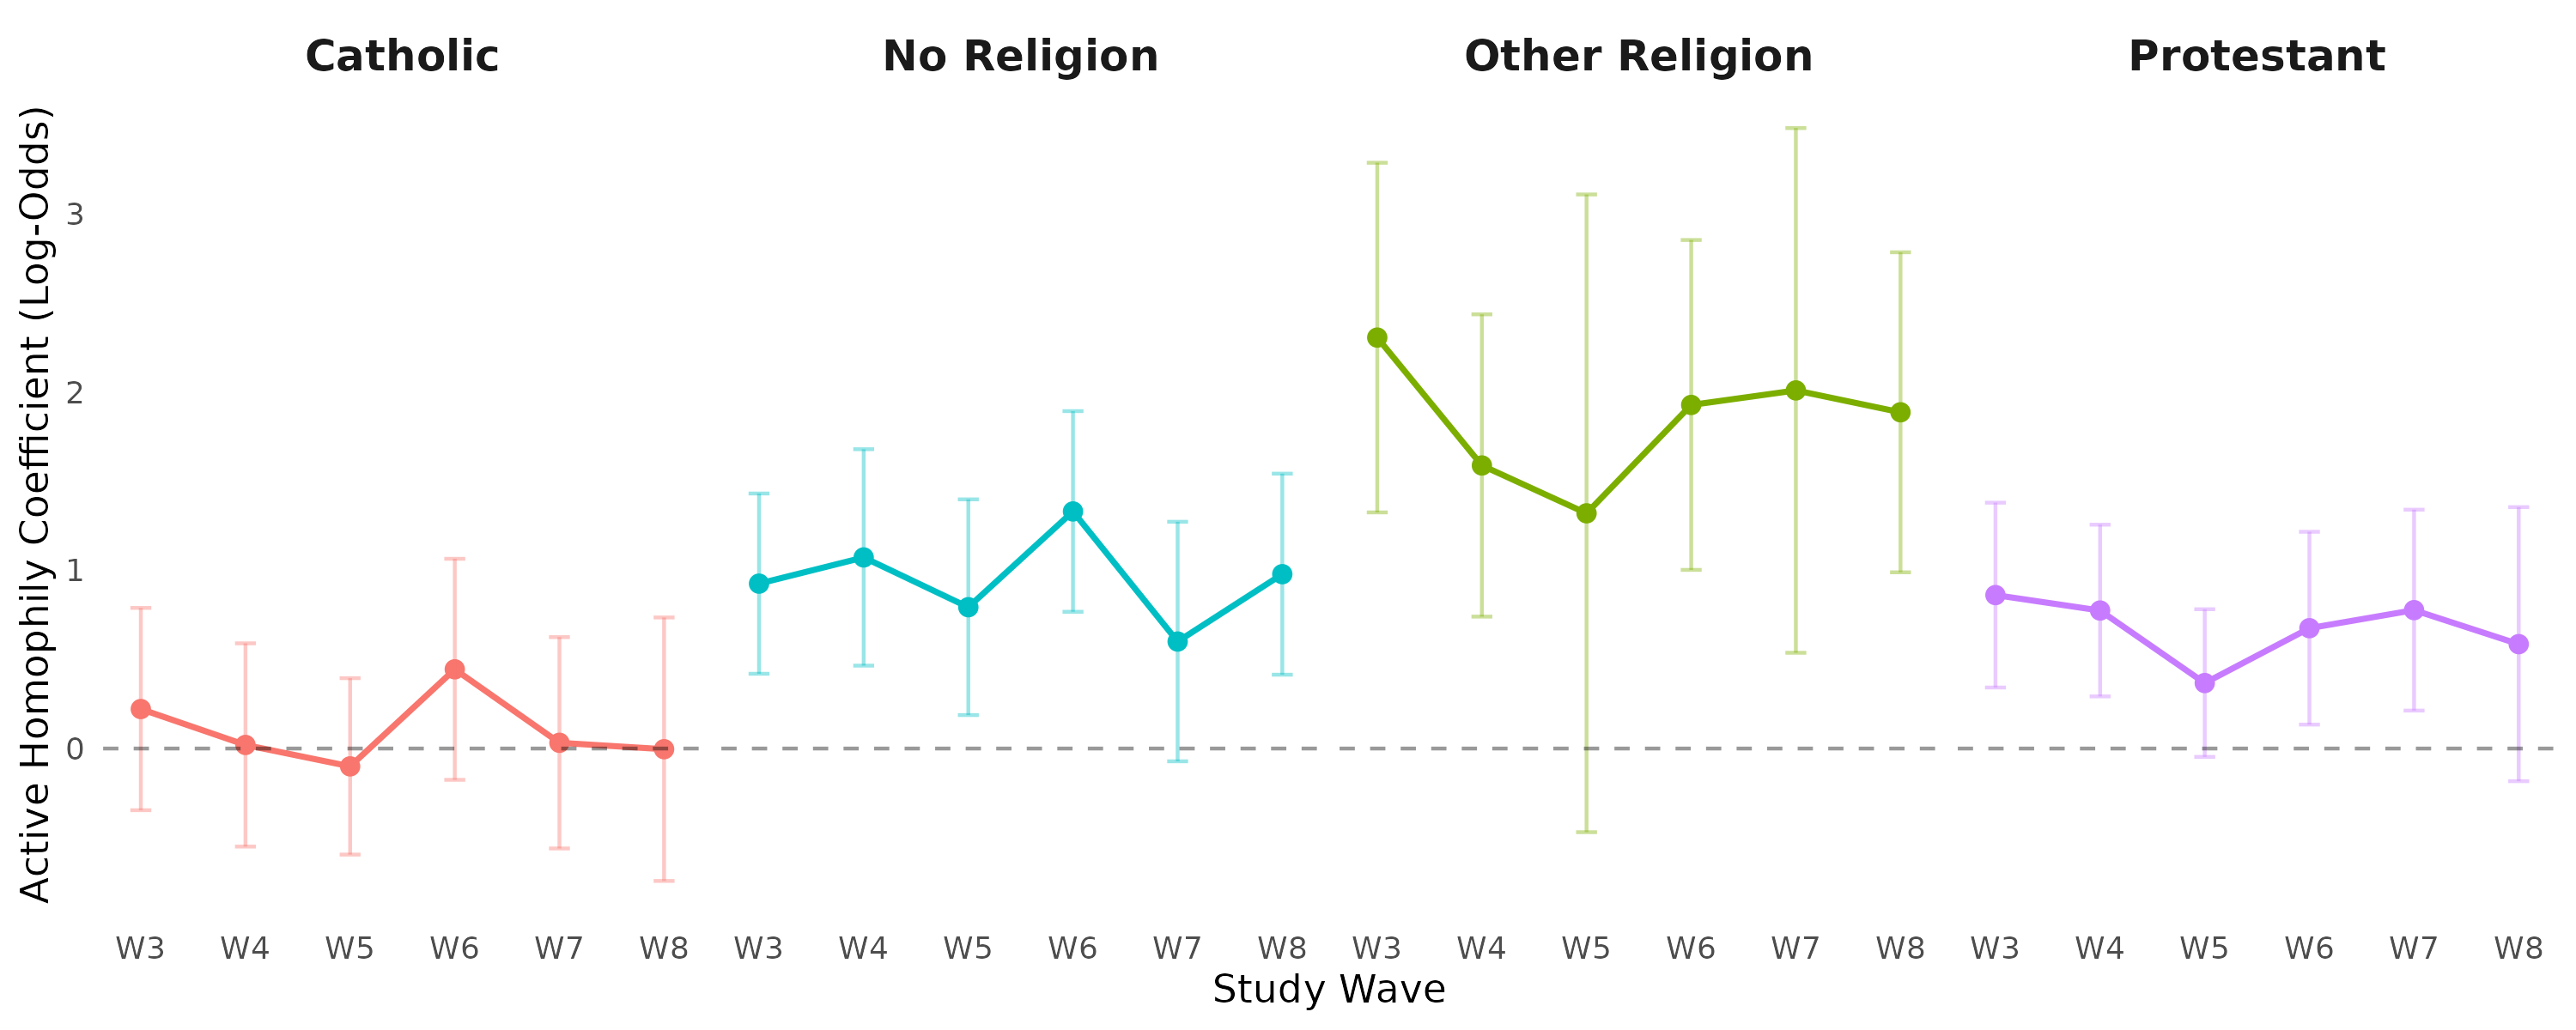
\includegraphics[width=1.0\textwidth]{Plots/fig-active-coefs.png}
    \caption{Active (Opportunity-Adjusted) Homophily Coefficients over Time (Waves 3-8).}
    \label{fig:active-coefs}
\end{figure}



\end{document}
